\documentclass[journal, onecolumn, 11pt]{IEEEtran}
\usepackage{mathtools}
\usepackage{graphicx}
\usepackage{amssymb}
\usepackage{amsmath}
\usepackage{pythonhighlight}
\usepackage[utf8]{inputenc}
\usepackage{fancyhdr}
\usepackage{pythonhighlight}
\usepackage{changepage}
\usepackage{slashbox}
\usepackage{floatrow}
\usepackage{listings}
\usepackage[hidelinks]{hyperref}
\usepackage{fontawesome}
\usepackage{caption}
\usepackage{subcaption}
\usepackage{cleveref}
\usepackage[style=ieeetran,style=numeric,sorting=none]{biblatex}
\addbibresource{references.bib}
\usepackage{color} 
\usepackage[english]{babel}
\usepackage{amsthm}
\usepackage{makecell}
\usepackage{diagbox}
\newtheorem{theorem}{Theorem}
\usepackage{multicol}
\newcommand{\Fourier}{$\mathcal{F}$}
\newcommand{\FourierAdj}{$\mathcal{F}^\ast$}

\author{Kutay Ugurlu}
\title{Analysis of Deep Convolutional Neural Network for Inverse Problems in Imaging
}
\begin{document}
\maketitle
\tableofcontents
\listoffigures
\listoftables
\clearpage

\section{Introduction}
In this term project report, the study \textit{Analysis of Deep Convolutional Neural Network for Inverse Problems in Imaging} by Jin \textit{et al.} \cite{FBPConvNet} is going to be reviewed, the results are going to reproduced and the experiments are going to be conducted using another dataset which is going to be formed by hand. 

The authors of the paper propose a convolutional neural network architecture mainly for the inverse problem of computerized tomography(CT) problems, while they stress that the proposed method is available for all normal-convolutional inverse problems. The study aims reconstructing the image from lower views by direct inversion followed by a convolutional neural network, more specifically a U-Net \cite{ronneberger2015u} based architecture. Starting from the observation that the normal operator $H^\ast H$, where $H^\ast$ is the adjoint operator of H that satisfies the relation $\langle f,H^\ast g \rangle = \langle Hf,g \rangle$, that appears as a forward model in a set of inverse problems, the authors investigate the relationship between the CNN models and the iterative optimization models utilized in inverse problems.  

\section{Theory}

\subsection{Shift-invariant Normal Operator}

To define a shift-invariant normal operator, the authors made the following definitions for the continuous domain: 
\begin{enumerate}
    \item \textit{Isometry:} An isometry $T$ is a linear operator such that $T^\ast T {f}(x) = f(x)$
    \item \textit{Multiplication:} A multiplication $M_m$ is a linear operator such that $M_m{f}(x) = m(x)f(x)$ where $m(x)$ is a continuous and bounded function.  
    \item \textit{Convolution:} A convolution $H_h$ is a linear operator such that $H_hf = \mathcal{F}^\ast M_{\hat{h}} \mathcal{F} f$ where $\mathcal{F}$ is the Fourier transform and $\hat{h}$ is the Fourier transform of h. 
    \item \textit{Reversible Change of Variables:} A reversible change of variables $\Phi_\psi: L_2(\Omega_1) \rightarrow L_2(\Omega_2)$ is a linear operator such that $\Phi_\phi f = f(\phi(.))$ for some $\phi: \Omega_2 \rightarrow \Omega_1$ and such that its inverse exists. That is, it is a linear operator that represents the same function via a reversible domain transformation, such as Cartesian to Polar coordinate transformation. 
\end{enumerate}

\begin{theorem}
    If an operator is in the form $H = TM_m{\Phi_\phi}^{-1}\mathcal{F}$, then normal operator $H^\ast H$ represents a convolution operation with $|det J_\phi| M_{\Phi_\phi |m|^2}$
    \label{thrm:Theorem1}
\end{theorem}
where $J_\phi$ is the Jacobian matrix.

\begin{proof}
    \begin{align}
        H^\ast H &= \mathcal{F}^\ast ({\Phi_\phi}^{-1})^\ast \underbrace{M_m^\ast \underbrace{T^\ast T}_{I} M_m}_{M_{{|m|}^2}} {\Phi_\phi}^{-1} \mathcal{F} \label{eq:proof1}\\ 
        H^\ast H &= \mathcal{F}^\ast ({\Phi_\phi}^{-1}) M_{|m|}^2 {\Phi_\phi}^{-1} \mathcal{F} \label{eq:proof2}\\
        (\Phi_\phi^{-1})^\ast &= |det J_\phi|\Phi_\phi \label{eq:proof3}\\
        H^\ast H &= \mathcal{F}^\ast |det J_\phi| M_{\Phi_\phi|m|}^2  \mathcal{F} \label{eq:proof4}
    \end{align}
    where the definition \ref{eq:proof3} is used in \Cref{eq:proof4} where the order of the change of variables and multiplications are exchanged with a change of variables in the multiplying kernel. \Cref{eq:proof4} is a multiplication in Fourier domain and the inversion following it, hence it is a convolution.
\end{proof}

\subsection{Forward Model of X-Ray CT Problem}
The main focus of the paper is reconstructing the X-ray CT image from low-view projections. When we consider the forward model as the 2 dimensional X-Ray Transform $R: L_2()\mathbb{R}^2) \rightarrow L_2([0,2\pi) \times \mathbb{R})$, also known as Radon Transform, we can express it using Fourier Slice Theorem as follows: 
\begin{equation}
    R = T {\Phi_\phi}^{-1} \mathcal{F}
    \label{eq:RadonTransform}
\end{equation}


where the coordinate transformation operation is defined as conversion from Cartesian to polar coordinates and $T$ is inverse Fourier transform with respect to 2D Fourier transform's radial variable $w$. The operation expressed by Eqn. \ref{eq:RadonTransform} takes the Fourier transform of the image, express the resultant signal in polar coordinates ($\Phi^{-1}(\theta, r) = (r\cos\theta,r\sin\theta)$) and takes the inverse Fourier transform. This process is equivalent to the operation of Projection Slice Theorem illustrated in \Cref{fig:radonimg}. Theorem \ref{thrm:Theorem1} states that $R^\ast R$ is a convolution with $\frac{1}{||w||}$ where w is the frequency variable for the 2D Fourier transform and $M_m$ in \Cref{thrm:Theorem1} is multiplication by identity. 

\begin{proof}
    \begin{align}
        R &= T {\Phi_\phi}^{-1} \mathcal{F} \\
        R^\ast R &=  \mathcal{F}^\ast |det J_\phi| \mathcal{F} \ \ (\ref{eq:proof4}) \\
    \end{align}
    where $det J_\Phi$ is $\frac{1}{||r||}$ in the polar space domain and $det J_\Phi(w)$ is $\frac{1}{||w||}$ in polar frequency domain.
\end{proof}

\begin{figure}[h]
    \centering
    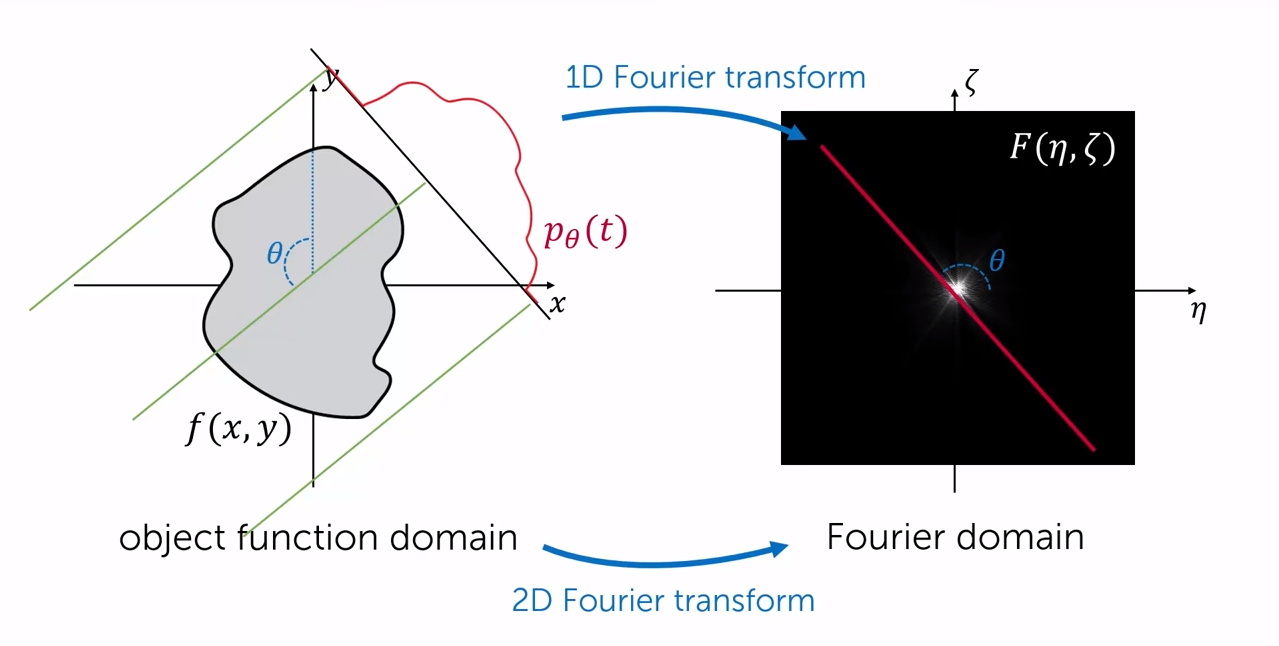
\includegraphics[width=0.8\textwidth]{images/slicethm.png}
    \caption{Projection slice theorem's illustration \cite{kooi_2021}}\label{fig:radonimg}
    \end{figure}
\subsection{Direct Inversion}

One may apply direct inversion methods to solve the inverse problem of tomography, \textit{i.e.}, obtaining the image from measurements. The problem can be formulated as $g=Hf$ where $H$ is a normal convolutional operator. According to \cite{FBPConvNet}, the solution can be obtained by direction inversion in two ways as follows: 

\begin{align}
    f &= W_h H^\ast g \label{eq:inv1}\\
    f &= H^\ast T M_h T^\ast g \label{eq:inv2}
\end{align}

where $W_h$ in \Cref{eq:inv1} is the convolution operator with $\frac{1}{|det J_\phi|\Phi_\phi|m(w)|^2}$ and $M_h$ is $\frac{1}{|det J_\phi||m(w)|^2}$. The physical interpretation behind these equations can be considered as follows: The operation in \Cref{eq:inv1} corresponds to the deconvolution in the reconstruction space, whereas \Cref{eq:inv2} corresponds to a filtering operation in Fourier domain followed by a back- projection, if $T$ is Fourier transform, which is called filtered back projection(FBP) where the projections are filtered with $||w||$ in the 2D polar Fourier transform domain. 

\subsection{Iterative Inversion}

There also exist iterative approaches to solving inverse problems and they are formulated as follows: 

\begin{equation}
    \operatorname*{argmin}_a ||y-HWa||_2^2 + \lambda ||a||_1 
    \label{eq:TV}
\end{equation}

where $x = Wa$ and $a$ is a sparse representation of x in a domain where x is transformed to by $W$. Since, this formulation does not produce a closed form solution, the equation is solved iteratively. 

\begin{figure}[h]
\centering
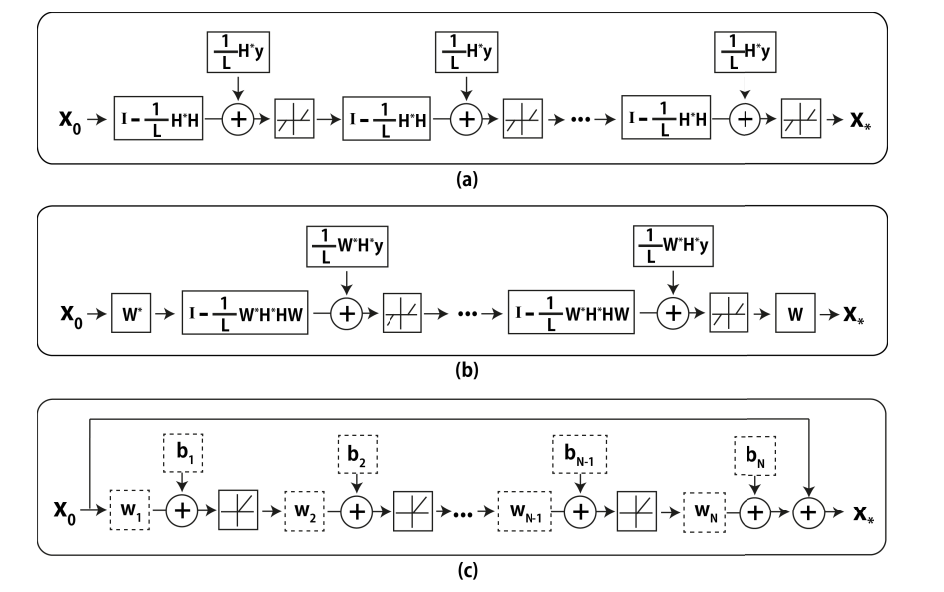
\includegraphics[width=\textwidth]{images/ISTA_block.png}
\caption{Block diagrams \cite{FBPConvNet} for (a) unfolded version \cite{ISTAnew} of iterative shrinkage method \cite{ISTA} with sparsifying transform W (b) and the corresponding block for CNN (c), where L is the Lipschitz constant, $x_0$ is the initial estimates,$b_i$ is the learned bias and $w_i$ is the trainable weights.}\label{fig:blocks}
\end{figure}

In Figure \Cref{fig:blocks}, the authors focus on the iterative procedures that utilizes sparsifying transforms and investigate the relationship between using the CNN and these methods. In (a) of \Cref{fig:blocks}, we observe that every iteration we encounter the normal operator. In (b), where a sparsifying transformation is used, we again have the normal operator in the unrolled iteration steps. These blocks including filtering by an operator that includes the normal operator along with the sparsifying transformation which usually can be expresseda s convolutions, an additive bias per each iteration followed by a pointwise nonlinearity.  

\vfill\null\newpage
\section{Proposed Method: FBPConvNet}

The authors state that the filtering and pointwise linearity operations in the iterative reconstruction methods may suggest that CNNs may be a good fit for the solution of the inverse problems. 
\\
\\
The approach simply consists of applying a direct inversion method to the measurements (sinograms in CT case) by Matlab's \texttt{iradon} function and feed the resultant projections to the CNN to train the network to learn the mapping between the back projected measurements and suitable ground truth images. 
The authors explain the reason for using a direct inversion method, instead of following an end-to-end neural net training approach between measurements and ground truth images as follows: 
By projecting the measurements to image domain, the learning is greatly simplified due to the fact that the network does not have to learn the coordinate transformation between Cartesian and Polar space. Since, filtered back projection encapsulates this operation and the physical information about the forward model. 

\subsection{Neural Network Model}

The design of the proposed network was based on U-Net. The modified architecture is illustrated in \Cref{fig:Unet}.

\begin{figure}[h]
\centering
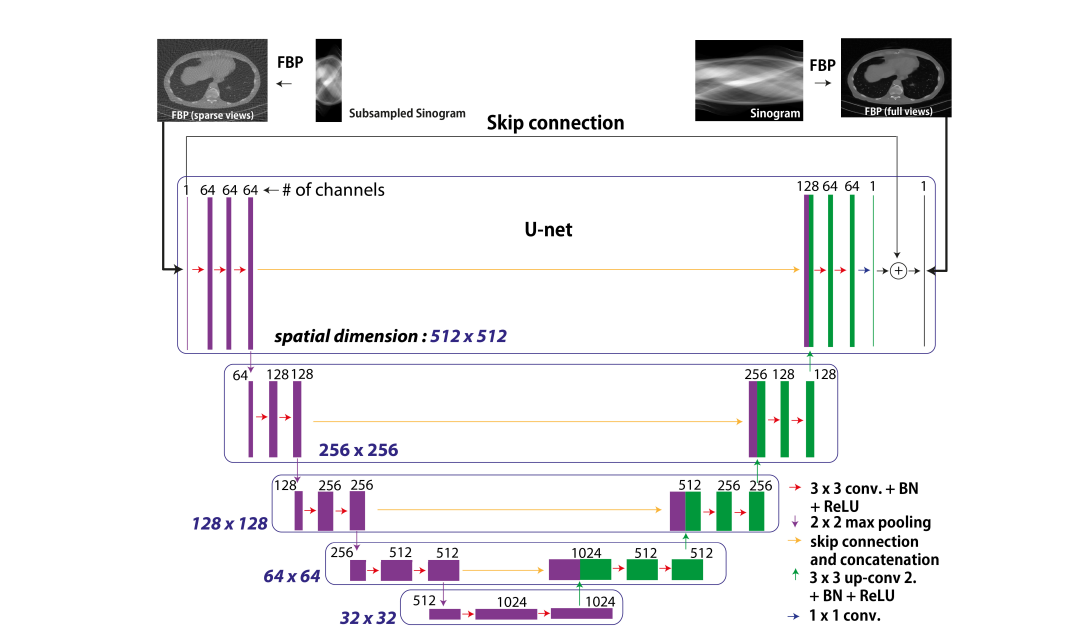
\includegraphics[width=0.8\textwidth]{images/unet.png}
\caption{Modified U-Net Architecture}\label{fig:Unet}
\end{figure}

The authors summarized the reasons for basing their architecture on U-Net as follows: 
\begin{itemize}
    \item \textit{Multilevel Decomposition:} The use of convolut The use of pooling kernels with different sizes help the network effectively invert $H^\ast H$. The usage of pooling makes the effective filter sizes in the middle layers larger than that of earlier and later layers. If the normal operator has a non-compact support, the different sizes of Fourier transforms corresponding to these different sizes provide more level of decompositions.
    \item \textit{Multichannel filtering:} The convolutional kernels have the ability to make arbitrary combinations of channels, analogous to wavelet subbands in ISTA or split variables in ADMM, that computes the solution in multiple channels or split variables. 
    \item \textit{Skip Connection for residual learning:} In addition to the original U-Net work, the authors added a skip connection between the input and output, allowing the network to learn the difference between the input and output. These connections have significant improvement in overcoming the gradient vanishing problem. 
    \item \textit{Last Layer:} The last layer of the network is replaced with a 1 $\times$ 1 convolution layer, since the original U-Net implementation has 2 channels: foreground and background. 
\end{itemize}

\subsection{Experiments}

Jin \textit{et al.} begin the reconstruction via full view sinogram from both real and simulated data. Then the reconstruction is performed on the subsampled sinogram. This type of procedure holds an important place in human imaging because lowering the views lower the radiation dose received by the patient. The full-view filtered back projection data is used as ground truth images, rather than the actual image, since the authors point out that this is a more realistic setting in practice since the oracle information will never be available in CT. The results are compared with the filtered back projection and method introduced in \cite{mccann2016fast} that solves \Cref{eq:TV} via ADMM. 

\subsection{Training the Network}

\subsubsection{Data}
The sample size of the train and test splits of the datasets are given in \Cref{tab:dataset}. 

\begin{table}[h]
    \centering
        \caption{Sample size for Datasets}
\begin{tabular}{|c|c|c|c|}
\hline 
\diagbox{Dataset}{Split} & \makecell{Training Data} & \makecell{Test Data} & Total \\ 
\hline 
Ellipsoid & 475 & 25 & 500 \\ 
Biomedical & \makecell{Scans from subjects \\ except one} & \makecell{Scans from the \\remaining subject} & 500 \\ 
Experimental & 327 & 25 & 377 \\ \hline 
\end{tabular}
    \label{tab:dataset}
\end{table}

The sinograms for ellipsoid dataset comprises of ellipses of random intensity, size and location. For the FBP implementation MATLAB's \texttt{iradon} function was utilized in both the original and replicated study. Sinograms for this dataset are 729 pixels by 1000 view. The biomedical dataset is from the Low-dose Grand challenge competition made by Mayo clinic and test data is formed by the scan of a subject whose scans were not in the training data. The sinograms are generated by the same approach in ellipsoid dataset. The experimental dataset comprises 377 sinograms from a real CT dataset collected from an experiment at the Paul Scherrer Institute. Each sinogram is 1493 pizels by 721 views and comes from one z-slice of a single rat brain. The image intensity dynamic range is set between -500 and 500.

\subsubsection{Training Procedure}

\begin{figure}[h]
    \centering
    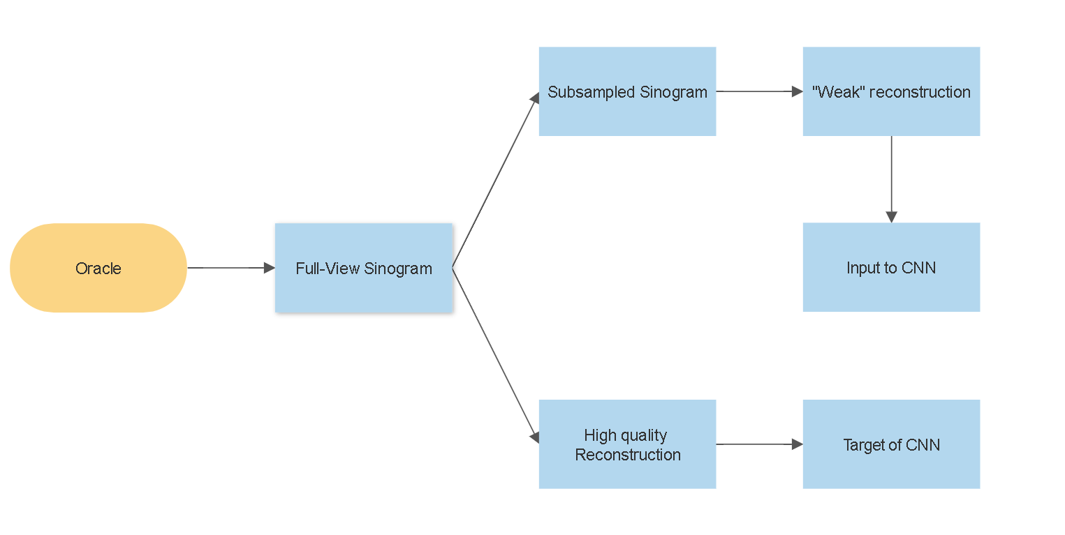
\includegraphics[width=0.8\textwidth]{images/IFLOW.png}
    \caption{Information flow in the proposed framework}\label{fig:iflow}
\end{figure}


The proposed CNN is trained with pairs of low view and full view FBP images (see \Cref{fig:iflow}) in MATLAB R2022(The MathWorks, Inc., Natick, Massachusetts, United States) using MatConvNet \cite{vedaldi2015matconvnet}. To reduce the overfitting, data augmentation is realized by mirroring the images in both vertical and horizontal directions. The training hyperparameters are set as follows: 

\begin{itemize}
\begin{multicols}{3}
    \item Gradient clipping: $10^{-2}$.
    \item Learning rate: [0.01,0.001]
    \item Loss: MSE (Euclidean Loss)
    \item Batchsize: 1
    \item Momentum: 0.99
    \item Optimizer: SGD
    \end{multicols}
\end{itemize}

The hyperparameters batchsize and learning rate are updated in the most recent repository.

\section{Results and Discussion}

\subsection{Reconstruction Performance Metrics}
The authors use SNR as a quantitative metric. The SNR of the reconstruction $\hat{x}$ with the ground truth image $x$ is given by \Cref{eqn:SNR}.

\begin{equation}
    SNR = \operatorname*{max}_{a,b \in \mathbb{R}} \frac{||x||_2}{||x - a\hat{x} + b||_2}
    \label{eqn:SNR}
\end{equation}

\subsection{Sample Reconstructions}

% \begin{figure}[h]
% \centering
% 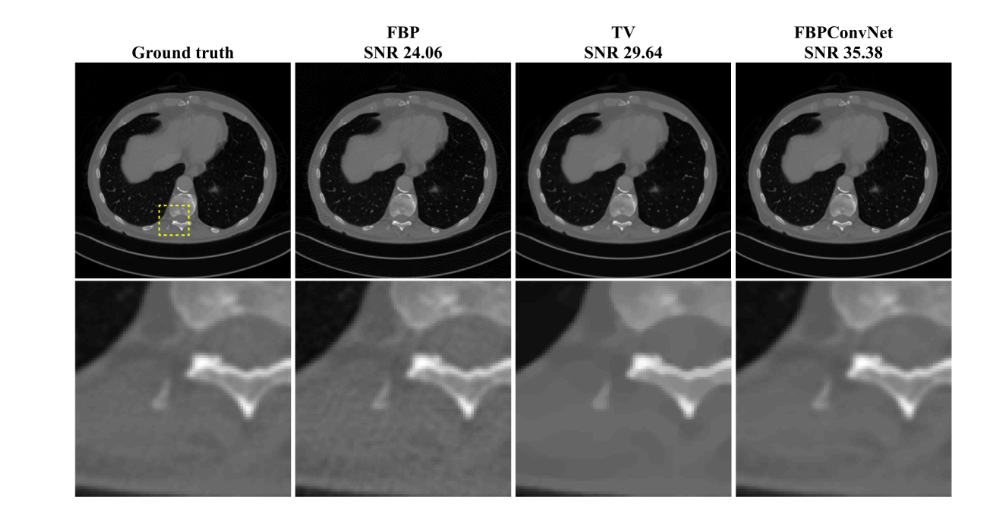
\includegraphics[width=0.8\textwidth]{images/results1.png}
% \caption{Reconstructed images of biomedical dataset from 143 views}\label{fig:res1}
% \end{figure}

% \begin{figure}[h]
%     \centering
%     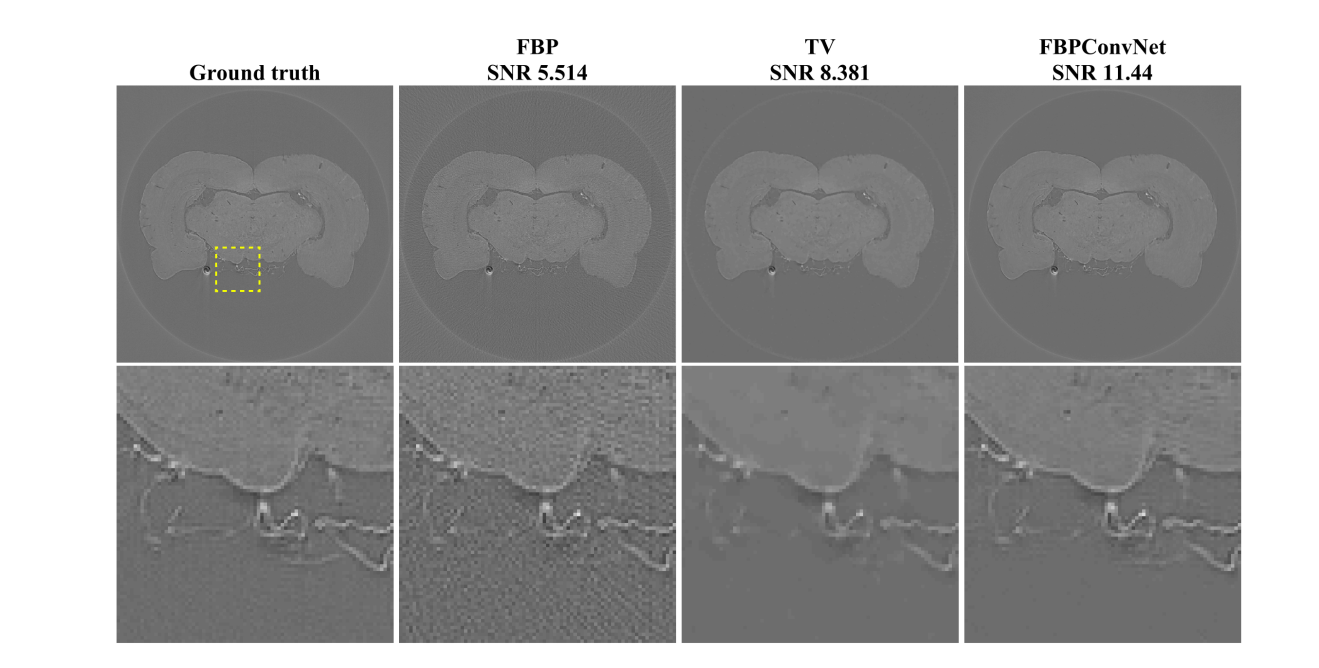
\includegraphics[width=0.8\textwidth]{images/results2.png}
%     \caption{Reconstructed images of experimental dataset from 145 views}\label{fig:res2}
% \end{figure}

\begin{figure}[h]
\centering
\begin{subfigure}[b]{0.75\textwidth}
\centering
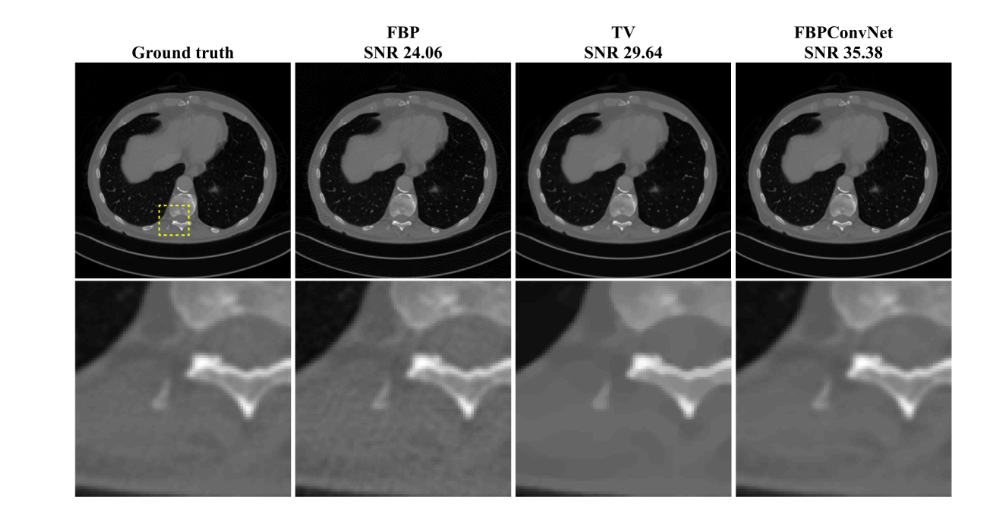
\includegraphics[width=\textwidth]{images/results1.png}
\caption{Biomedical Dataset: 50 views}\label{subfig:a}
\end{subfigure}
\\
\begin{subfigure}[b]{0.75\linewidth}
\centering
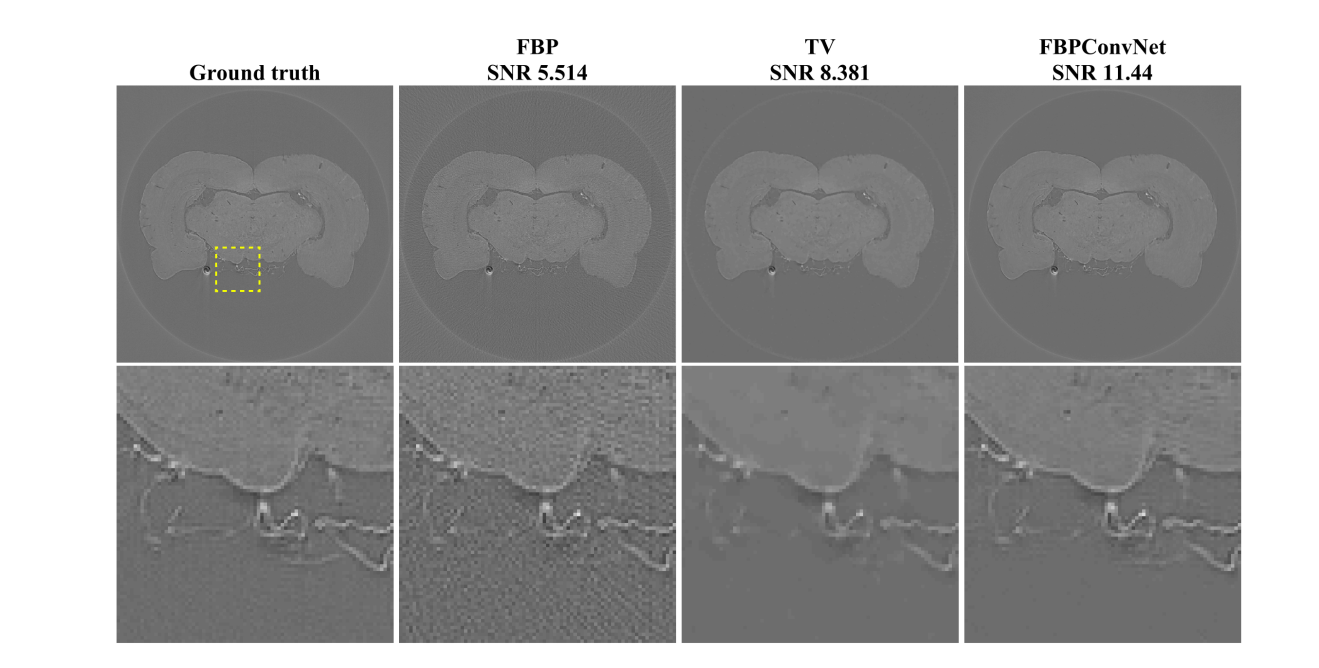
\includegraphics[width=\textwidth]{images/results2.png}
\caption{Experimental Dataset: 145 views}\label{subfig:b}
\end{subfigure}
\caption{Reconstruction comparisons for different datasets}
\label{fig:recs}
\end{figure}

The results of the experiments showed that the choice of CNN for the set of inverse problems where the forward model is convolution is suitable. In both \Cref{subfig:a} and \Cref{subfig:b} the reconstruction performance of the FBPConvNet against back projection can be observed qualitatively. The proposed method yields compelling results in both real and synthetic data. It outperformed iterative reconstruction method \cite{TV}. For a subsampling factor of 7 (143 views) the SNR of the recostructed image is 35.58dB SNR whereas for subsampling factor of 20 (50 views) it was 11.44 dB SNR. 

\begin{table}[h]
\caption{\label{tab:res1}Results for Biomedical Dataset}
\centering{
\begin{tabular}{|c|ccc|} \hline
    \diagbox{Metrics}{Methods} & FBP & TV \cite{TV} & FBPConvNet \\ \hline
    SNR for 143 views & 24.97 & 31.92 & 36.15 \\
    SNR for 50 views & 13.52 & 25.2 & 28.83 \\ \hline
\end{tabular}}
\end{table}

\begin{table}[h]
    \caption{\label{tab:res2}Results for Experimental Dataset}
    \centering{
    \begin{tabular}{|c|ccc|} \hline
        \diagbox{Metrics}{Methods} & FBP & TV \cite{TV} & FBPConvNet \\ \hline
        SNR for 143 views & 5.38 & 8.25 & 11.34 \\
        SNR for 50 views & 3.29 & 7.25 & 8.85 \\ \hline
    \end{tabular}}
    \end{table}
    
As we observe in \Cref{tab:res2}, the performance of the proposed network is lower in the experimental dataset and for lower views. We are able to see this trend in \Cref{fig:compareview} where the network is trained with 143 views and tested with different views. We observe that the SNR of reconstruction drop monotonically with increasing subsampling factors of decreasing number of views. 

\begin{figure}[h]
\centering
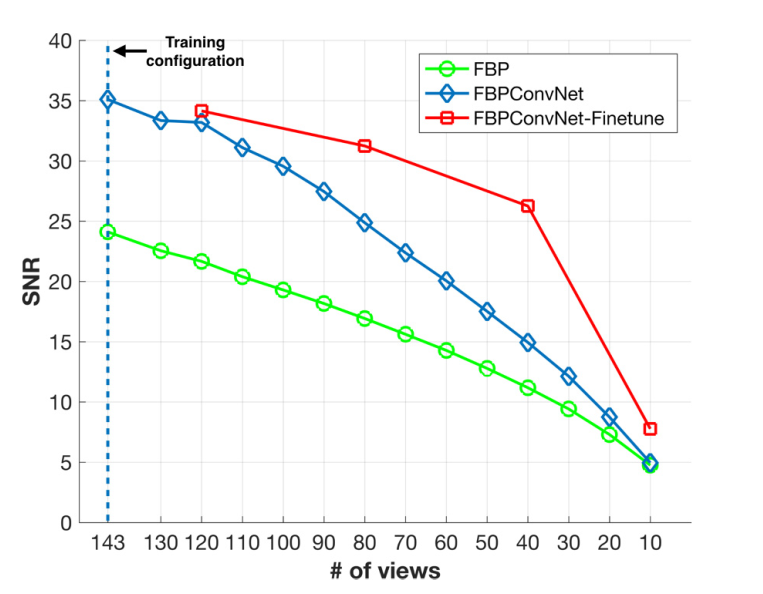
\includegraphics[width=0.6\textwidth]{images/viewscompare.png}
\caption{Performance with different number of views}\label{fig:compareview}
\end{figure}

\clearpage

\subsection{Replicated Experiment and Results} \label{subsec:training}

Two models are trained for 10 and 20 epochs with according scaled initial learning rates with respect to 100 epochs using the ellipsoid dataset provided in the original repository of the study, where the input images of the CNN are produced with FBP of the 50 view projections. The better model is used in the evaluation of different testing configurations. It is important to note that the network is undertrained when compared to the training configuration in the original study. 

\begin{figure}[h]
\centering
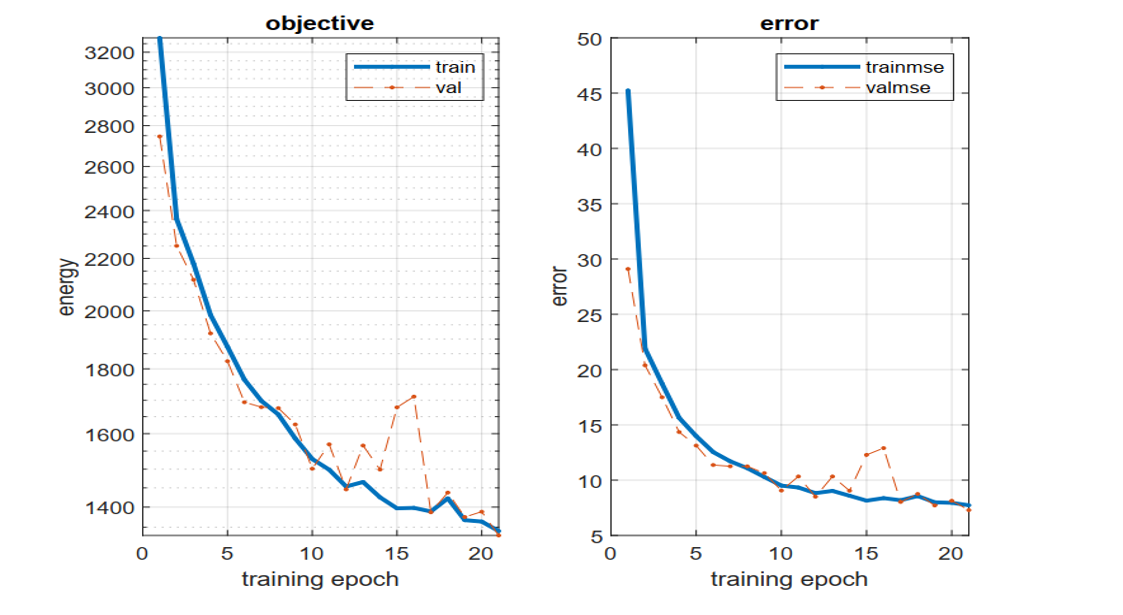
\includegraphics[width=0.6\textwidth]{images/training.png}
\caption{Training and Validation Losses for 20 epochs}\label{fig:training}
\end{figure}


\begin{figure}[h]
\centering
\begin{subfigure}[b]{0.8\linewidth}
\centering
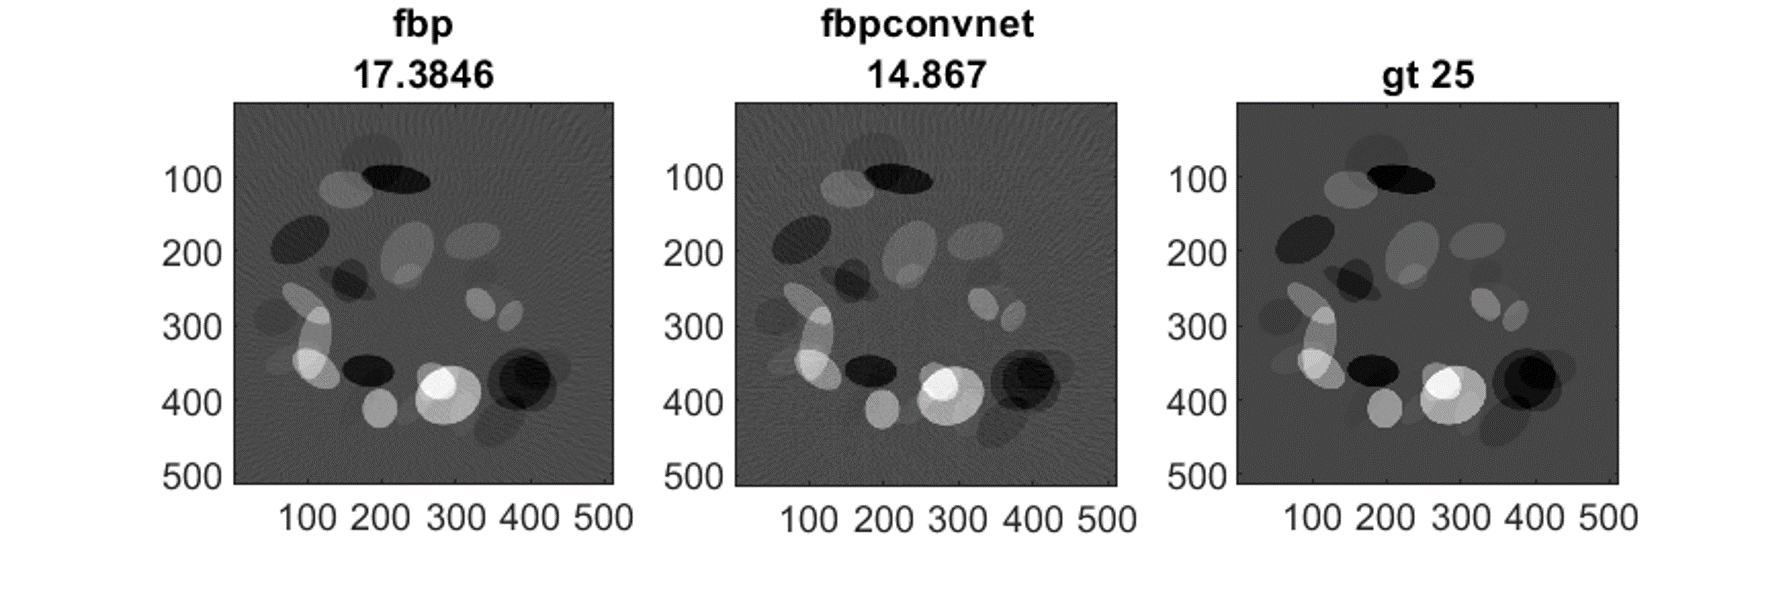
\includegraphics[width=\textwidth]{images/reprec10.png}
\caption{100 views}\label{subfig:2a}
\end{subfigure}
\begin{subfigure}[b]{0.8\linewidth}
\centering
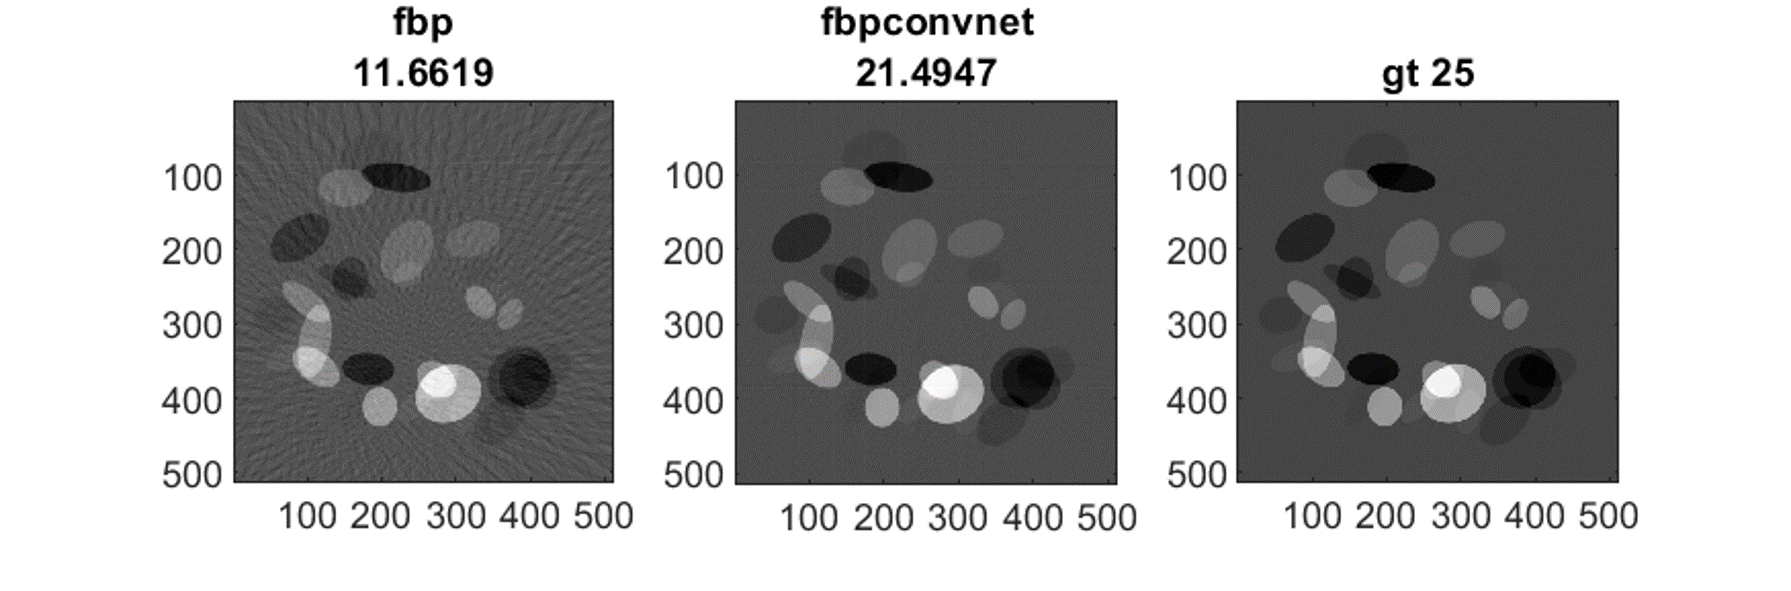
\includegraphics[width=\textwidth]{images/reprec20.png}
\caption{50 views}\label{subfig:2b}
\end{subfigure}
\caption{Reconstructions for different number of views}
\label{fig:reprecs}
\end{figure}

\vfill\null\newpage
\subsubsection{Testing on Ellipsoid Dataset}

Different sub-datasets are generated with noise and without noise and for different number of view angles using the ellipsoidal dataset to test the performance of the trained network. For the case illustrated in \Cref{fig:reprecs}, we observe that FBPConvNet generates outputs with SNRs 14.87 and 21.49 dB respectively. 


\begin{table}[h]
\centering{
\begin{tabular}{|c|c|c|c|c|} \hline
    \makecell{Experiment \\ Number} & \makecell{Subsampling \\ $\times N$} & \makecell{Noise \\ dB*} & \makecell{FBP \\ SNR(dB)} & \makecell{FBPConvNet \\ SNR(dB)} \\ \hline 
    1 & 10 & -  & 15.88 & 11.83 \\
    2 & 10 & 10 & 15.88 & 11.83 \\
    3 & 20 & -  & 10.21 & 17.48 \\
    4 & 20 & 10 & 10.21 & 17.48 \\
    5 & 25 & -  & 8.67  & 17.89 \\
    6 & 25 & 10 & 8.67  & 17.89 \\
    7 & 50 & -  & 4.83  & 8.48 \\
    8 & 50 & 10 & 4.83  & 8.48  \\\hline
\end{tabular}}
\caption{\label{tab:tabname}Experiment results for training configuration described in \Cref{subsec:training}. \newline * Noise SNR is described in \Cref{eq:noisesnr}}
\end{table}

\begin{equation}
    SNR_{noise}: \frac{P_{signal}}{P_{noise}} = \frac{\sum |signal|^2}{|noise|^2
    \label{eq:noisesnr}} 
\end{equation}

The experiments took 4 second per test image on CPU on average and they show that the trained model's performance peaks when  
the input images' sinogram subsampling matches that of images in the training set. This is why the SNR of the reconstruction SNR values of reconstructions from FBPConvNet exhibit a non-monotonic behavior, whereas the performance of FBP is decreasing monotonically with decreasing number of projection view angles. Furthermore, it is observed that the added 10 dB SNR noise did not affect the reconstructions in SNR sense in the given precision, although the network is trained with noise-free images. To compare with the original study, although undertrained, the model showed similar success for 50 view in the ellipsoid dataset. 

\subsubsection{Testing on SYNAPSE dataset}
To test the generalization of the trained network on another dataset, the synapse dataset is utilized \cite{SYNAPSE}. This dataset is from MultiAtlas Labelling Challenge and is for segmentation purposes. Since it is open access, images from the dataset are utilized which includes scans that adds up to 3779 axial contrast-enhanced CT images. 

\begin{figure}[h]
\centering
\begin{subfigure}[b]{\textwidth}
\centering
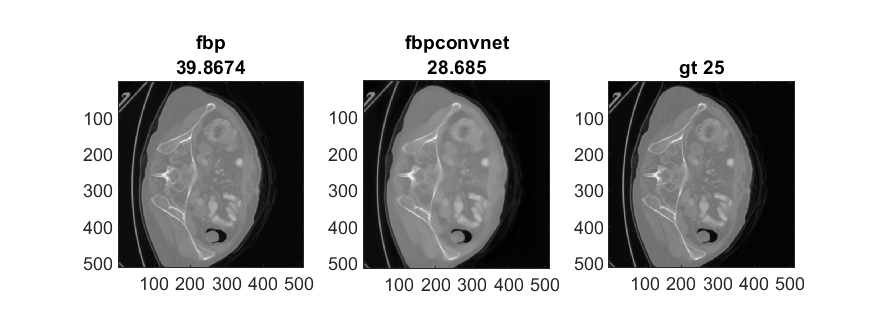
\includegraphics[width=0.8\textwidth]{images/SS2.png}
\caption{500 views}\label{subfig:3a}
\end{subfigure}
\begin{subfigure}[b]{\linewidth}
\centering
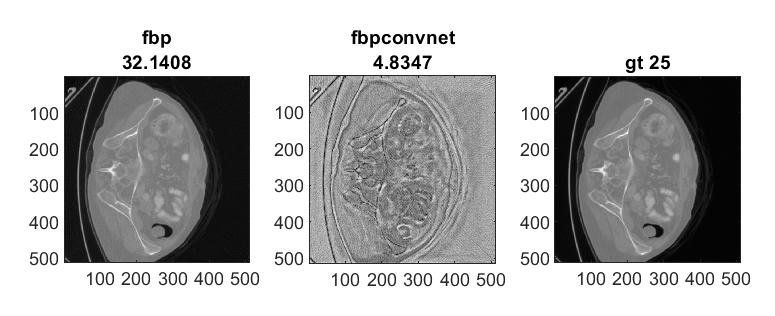
\includegraphics[width=0.7\textwidth]{images/SS5.png}
\caption{200 views}\label{subfig:3b}
\end{subfigure}
\begin{subfigure}[b]{\linewidth}
\centering
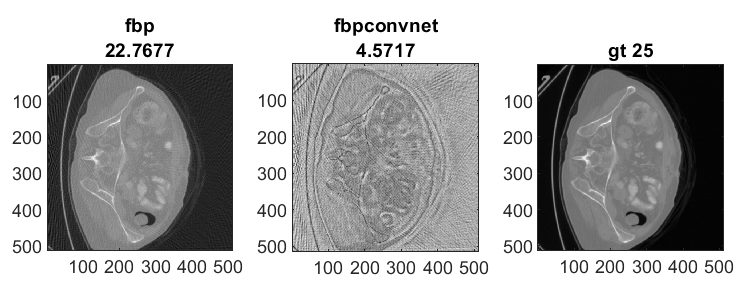
\includegraphics[width=0.7\textwidth]{images/SS10.png}
\caption{100 views}\label{subfig:3c}
\end{subfigure}
\caption{Reconstructions generated for SYNAPSE dataset for different number of views}
\label{fig:Synapses}
\end{figure}

The reconstructions from \Cref{fig:Synapses} show that the trained network does not only learn the convolutional filters that correspond to $R^\ast R$ for FBP of subsampled sinograms or their inverse. Instead, the model also learned how to remove the artifacts of the "weak" reconstructions from subsampled sinograms fitting to the prior distribution of the images in the ellipsoid dataset. 

\subsection{Conclusion}

In this project, the study \textit{Deep Convolutional Neural Network for Inverse Problems in Imaging} is analyzed using the software provided and some of the results are replicated using the provided preprocessed ellipsoid dataset. For the training configuration used to replicate the study, the network improved the images generated by FBP, outperforming it by approximately 9dB. For other subsampling factors and the same dataset, FBPConvnet output qualitatively acceptable images. 
\clearpage
\printbibliography

\end{document}